\documentclass[11pt,twocolumn]{article}

% ── Packages ──────────────────────────────────────────────────────────────────
\usepackage[margin=1in,top=1in,bottom=1in]{geometry}
\usepackage{amsmath,amssymb,amsthm}
\usepackage{graphicx}
\usepackage{booktabs}
\usepackage{array}
\usepackage{multirow}
\usepackage{hyperref}
\usepackage{url}
\usepackage{xcolor}
\usepackage{enumitem}
\usepackage{titlesec}
\usepackage{abstract}
\usepackage{microtype}
\usepackage{parskip}
\usepackage[ruled,vlined,linesnumbered]{algorithm2e}
\usepackage{caption}
\usepackage{subcaption}
\usepackage{float}
\usepackage{fancyhdr}
\usepackage{lipsum}
\usepackage{setspace}
\usepackage{cite}

% ── Hyperref colours ──────────────────────────────────────────────────────────
\hypersetup{
    colorlinks=true,
    linkcolor=blue!60!black,
    citecolor=blue!60!black,
    urlcolor=blue!60!black,
}

% ── Header / Footer ───────────────────────────────────────────────────────────
\pagestyle{fancy}
\fancyhf{}
\rhead{\small CSC 520 --- Final Project Report}
\lhead{\small Desemsetti}
\cfoot{\thepage}
\renewcommand{\headrulewidth}{0.4pt}

% ── Section title formatting ──────────────────────────────────────────────────
\titleformat{\section}{\large\bfseries}{{\thesection.}}{0.5em}{}[\titlerule]
\titleformat{\subsection}{\normalsize\bfseries}{{\thesubsection}}{0.5em}{}
\titleformat{\subsubsection}{\normalsize\itshape}{{\thesubsubsection}}{0.5em}{}

% ── Abstract formatting ───────────────────────────────────────────────────────
\renewcommand{\abstractnamefont}{\large\bfseries}
\renewcommand{\abstracttextfont}{\normalsize}

% ── Math helpers ──────────────────────────────────────────────────────────────
\newcommand{\argmax}{\operatorname{argmax}}
\newcommand{\Q}{Q}

% ─────────────────────────────────────────────────────────────────────────────
\begin{document}

% ── Title block ───────────────────────────────────────────────────────────────
\twocolumn[{%
\begin{@twocolumnfalse}

\begin{center}
    {\LARGE\bfseries Delivery Drone Route Planner:\\[4pt]
    A Two-Layer AI System Combining\\[4pt]
    Q-Learning Dispatch and A* Pathfinding}\\[14pt]

    {\large
        Srikar Desemsetti
    }\\[6pt]

    {\normalsize
        \texttt{spdesems@ncsu.edu}
    }\\[4pt]

    {\normalsize\itshape
        Department of Computer Science, North Carolina State University\\
        CSC 520: Artificial Intelligence \quad --- \quad Spring 2026
    }\\[12pt]
\end{center}

\begin{abstract}
\noindent
We present the \textbf{Delivery Drone Route Planner}, a two-layer autonomous
agent for multi-delivery drone routing on a stochastic city grid.
The high-level layer employs tabular Q-learning to select dispatch
decisions---which delivery to attempt, when to recharge, and when to
abandon a job---while the low-level layer executes each decision using
A* search with wind-penalised edge costs, battery-budget pruning, and
dynamic replanning around moving obstacles.
We evaluate the learned policy against a greedy nearest-neighbour baseline
and a random policy across 100 reproducible scenarios on three difficulty
tiers (easy, medium, hard).
On the easy tier, Q-learning achieves a delivery success rate of
\textbf{83.5\%}, marginally outperforming the greedy baseline (82.9\%) and
more than quadrupling the random policy (20.0\%).
Our results demonstrate that a tabular RL agent can match and slightly
surpass a carefully designed heuristic on small grids, while also
exposing well-known scalability limitations of tabular Q-learning on
larger state spaces.
\end{abstract}
\vspace{10pt}
\end{@twocolumnfalse}
}]

% ─────────────────────────────────────────────────────────────────────────────
\section{Introduction}
\label{sec:intro}
% ─────────────────────────────────────────────────────────────────────────────

Autonomous last-mile delivery has become an active research frontier as
commercial operators seek to reduce logistics costs and human labour.
Unmanned aerial vehicles (UAVs), or drones, are particularly appealing
because they operate independently of road congestion.
However, real-world drone routing is considerably harder than classic
single-vehicle routing: a drone must simultaneously manage limited battery
capacity, comply with dynamic airspace restrictions, avoid moving hazards,
and respect delivery deadlines---all in a partially observable and
stochastic environment.

This project addresses drone delivery routing as a two-level planning
problem.
At the \emph{strategic level}, the agent must decide \emph{what} to do
next: commit to a specific delivery, fly to a charging station, or
deliberately skip a job it cannot complete profitably.
At the \emph{tactical level}, the agent must decide \emph{how} to execute
that decision: compute an efficient, collision-free path through the city
while respecting battery constraints and reacting to obstacles that move
unpredictably.

We decompose this into two classical AI paradigms studied in this course:
\begin{enumerate}[leftmargin=*, nosep]
    \item \textbf{A* heuristic search}~\cite{hart1968} for optimal,
          battery-aware low-level path planning with dynamic replanning.
    \item \textbf{Tabular Q-learning}~\cite{watkins1992} for learning a
          high-level dispatch policy through trial-and-error interaction
          with a simulated city environment.
\end{enumerate}

The remainder of this report is organised as follows.
Section~\ref{sec:problem} formalises the problem.
Section~\ref{sec:approach} describes the technical approach.
Section~\ref{sec:experiments} details the experimental setup.
Section~\ref{sec:results} presents quantitative results.
Section~\ref{sec:discussion} interprets those results and discusses
limitations.
Section~\ref{sec:conclusion} concludes.

% ─────────────────────────────────────────────────────────────────────────────
\section{Problem Formulation}
\label{sec:problem}
% ─────────────────────────────────────────────────────────────────────────────

\subsection{Environment Model}

We model the delivery city as an $N \times N$ discrete grid.
Each cell is either \emph{open} or part of a \emph{no-fly zone} (NFZ).
A single drone starts at a randomly assigned cell with a full battery of
$B_{\max} = 100$ units.
The environment contains the following entities:

\begin{itemize}[leftmargin=*, nosep]
    \item \textbf{Deliveries} $\mathcal{D}$: a set of jobs, each with a
          dropoff cell $d_i$ and a time window $(t_i^{\min}, t_i^{\max})$.
          A delivery earns reward $+100$ if the drone reaches $d_i$
          within the window.
    \item \textbf{Charging stations} $\mathcal{C}$: cells that
          immediately restore battery to $B_{\max}$ upon landing.
    \item \textbf{Moving obstacles} $\mathcal{O}$: cells that relocate
          by one step each timestep.
          Collision results in a penalty of $-50$ and episode termination.
    \item \textbf{Wind map} $W$: a $2$-D array where $W[r][c] \in [0.5,
          2.0]$ is the wind factor at cell $(r,c)$, drawn from a clipped
          Gaussian $\mathcal{N}(1.0,\,0.04)$.
          Battery consumption per move is $\|u - v\|_2 \cdot W[v]$.
\end{itemize}

\subsection{Two-Level Decision Problem}

\paragraph{Low-level (path planning).}
Given a target cell $g$, find a sequence of cells from the drone's
current position to $g$ that minimises battery cost subject to NFZ
avoidance and battery feasibility.
If a moving obstacle blocks the planned route mid-flight, the path is
immediately replanned.

\paragraph{High-level (dispatch).}
Given the full world state, select the next \emph{macro-action}: fly to
a delivery dropoff, fly to a charging station, or skip a delivery.
This is modelled as an MDP (Section~\ref{sec:mdp}).

\subsection{Markov Decision Process}
\label{sec:mdp}

The high-level dispatch problem is formalised as a finite MDP
$\langle \mathcal{S}, \mathcal{A}, T, R, \gamma \rangle$.

\paragraph{State space $\mathcal{S}$.}
To keep the Q-table tractable we discretise continuous quantities:
\begin{align}
s = \bigl(&\text{drone\_pos},\;
           b_{\text{bin}},\;
           \text{remaining},\;
           t_{\text{bin}}\bigr),
\end{align}
where $\text{drone\_pos} \in \{0,\ldots,N-1\}^2$ is the current cell,
$b_{\text{bin}} = \lfloor B / 10 \rfloor \in \{0,\ldots,10\}$ is a
coarse battery level, $\text{remaining} \subseteq \mathcal{D}$ is the
\texttt{frozenset} of pending delivery IDs, and $t_{\text{bin}} = \lfloor
10 \cdot t / T_{\max} \rfloor \in \{0,\ldots,9\}$ is a coarse time
fraction.

\paragraph{Action space $\mathcal{A}$.}
Three macro-action types are available:
\begin{itemize}[leftmargin=*, nosep]
    \item \textsc{Deliver}$(i)$: route to delivery $i$'s dropoff cell.
    \item \textsc{Charge}: route to the nearest charging station.
    \item \textsc{Skip}$(i)$: mark delivery $i$ as failed; no movement.
\end{itemize}
Only actions consistent with the current state (e.g.\ only pending
deliveries can be targeted) appear in the valid action set.

\paragraph{Reward function.}
The per-step reward is
\begin{equation}
r_t = -1 + 100 \cdot \mathbb{1}[\text{on-time delivery}]
           - 50  \cdot \mathbb{1}[\text{crash}].
\end{equation}

\paragraph{Discount factor.}
We use $\gamma = 0.95$, giving near-equal weight to short- and
medium-term outcomes while ensuring convergence.

% ─────────────────────────────────────────────────────────────────────────────
\section{Technical Approach}
\label{sec:approach}
% ─────────────────────────────────────────────────────────────────────────────

\subsection{Layer 1 --- A* Pathfinding}
\label{sec:astar}

A* search~\cite{hart1968} is a best-first graph search algorithm that
finds the minimum-cost path from a start node to a goal node by
evaluating
\begin{equation}
    f(n) = g(n) + h(n),
\end{equation}
where $g(n)$ is the cost accumulated from the start to node $n$ and
$h(n)$ is an admissible heuristic estimating the remaining cost.

\subsubsection{Heuristic design.}
The drone moves in eight directions (cardinal and diagonal).
The cost of a cardinal step is $1.0$ and of a diagonal step is
$\sqrt{2}$, scaled by the destination wind factor.
We use Euclidean distance as the heuristic:
\begin{equation}
    h(n) = \|(n_r - g_r,\; n_c - g_c)\|_2.
\end{equation}
Euclidean distance is \emph{admissible} for 8-directional grids because
the true path cost is always at least the straight-line distance.
It is also \emph{consistent} (monotone): $h(n) \leq c(n,n') + h(n')$
for every edge $(n,n')$, ensuring that each node is expanded at most
once.

\subsubsection{Battery-constrained pruning.}
Any partial path whose accumulated cost exceeds the remaining battery
$B_{\text{rem}}$ is pruned during expansion.
This transforms A* into a battery-aware planner without modifying the
core algorithm: the search simply never opens nodes that are battery-
infeasible.

\subsubsection{Wind-penalised edge costs.}
Moving from cell $u$ to adjacent cell $v$ costs
\begin{equation}
    c(u, v) = \|u - v\|_2 \cdot W[v],
\end{equation}
where $W[v] \in [0.5, 2.0]$ is the per-cell wind factor.
High-wind cells effectively repel the planner: A* may route around a
high-wind zone even when the direct path through it is shorter in
Euclidean distance.

\subsubsection{Dynamic replanning.}
After each simulator step, we invoke \texttt{replan()}, which checks
whether any cell in the drone's remaining planned path has become
occupied by a moving obstacle.
If a conflict is detected, A* is re-invoked from the drone's current
position.
This is a form of \emph{incremental replanning}~\cite{likhachev2005}:
the system does not replan from scratch every step, but only when the
environment invalidates the current plan.

Algorithm~\ref{alg:astar} summarises the A* implementation.

\begin{algorithm}[H]
\small
\caption{A* with battery pruning and wind costs}
\label{alg:astar}
\SetAlgoLined
\KwIn{grid $G$, start $s$, goal $g$, NFZs, wind map $W$, battery $B$}
\KwOut{(path, cost) or \texttt{None}}
Open $\leftarrow$ min-heap$\{(f(s), 0, s, [s])\}$\;
$g\_cost[s] \leftarrow 0$\;
\While{Open $\neq \emptyset$}{
    $(f, cost, n, \text{path}) \leftarrow$ \texttt{heappop}(Open)\;
    \lIf{$cost > g\_cost[n]$}{\textbf{continue} \tcp*{stale entry}}
    \lIf{$n = g$}{\Return (path, cost)}
    \ForEach{neighbour $v$ of $n$}{
        \lIf{$v \in$ NFZ or $v \in$ obstacle}{\textbf{continue}}
        $c' \leftarrow cost + \|n{-}v\|_2 \cdot W[v]$\;
        \lIf{$c' > B$}{\textbf{continue} \tcp*{battery pruned}}
        \If{$c' < g\_cost[v]$}{
            $g\_cost[v] \leftarrow c'$\;
            $f' \leftarrow c' + \|v{-}g\|_2$\;
            \texttt{heappush}(Open, $(f', c', v, \text{path}+[v])$)\;
        }
    }
}
\Return \texttt{None}\;
\end{algorithm}

\subsection{Layer 2 --- Tabular Q-Learning}
\label{sec:qlearning}

Q-learning~\cite{watkins1992} is a model-free, off-policy reinforcement
learning algorithm that directly estimates the optimal state-action value
function $Q^*(s,a)$ satisfying the Bellman optimality equation:
\begin{equation}
    Q^*(s,a) = \mathbb{E}\!\left[r + \gamma \max_{a'} Q^*(s',a')\right].
\end{equation}

\subsubsection{Update rule.}
After observing transition $(s, a, r, s')$, the Q-table is updated as
\begin{equation}
    Q(s,a) \;\leftarrow\; Q(s,a) + \alpha\,\bigl[\,r + \gamma
    \max_{a'} Q(s',a') - Q(s,a)\,\bigr],
    \label{eq:qupdate}
\end{equation}
with learning rate $\alpha = 0.1$ and discount $\gamma = 0.95$.
Unvisited $(s,a)$ pairs default to $Q = 0$.

\subsubsection{Exploration.}
We use an $\varepsilon$-greedy policy:
\begin{equation}
    a_t = \begin{cases}
        \text{random valid action} & \text{with prob.\ } \varepsilon, \\
        \argmax_{a} Q(s_t, a) & \text{otherwise.}
    \end{cases}
\end{equation}
$\varepsilon$ decays linearly from $1.0$ to $0.05$ over the full
training run, balancing early exploration against late exploitation.

\subsubsection{Sparse Q-table.}
The Q-table is implemented as a nested \texttt{defaultdict}: only
$(s,a)$ pairs visited during training occupy memory.
This is critical for tabular methods because the theoretical state space
is exponentially large in the number of deliveries.
After 5\,000 episodes the table contains on the order of $10^3$--$10^4$
visited states for the easy tier.

\subsubsection{Episode diversity.}
Each training episode uses a distinct random seed
$\sigma_k = \sigma_0 + k$, so the agent trains on varied city layouts,
wind maps, and obstacle configurations.
Without seed variation, the agent would memorise a single map rather
than learning a generalisable dispatch policy.

\subsubsection{SKIP as a strategic action.}
The \textsc{Skip} action allows the drone to deliberately abandon a
delivery.
This is not a failure mode---it is a learned strategy.
When a delivery is far away and the time window is tight, the cost of
attempting it (battery expenditure, time elapsed) may exceed the expected
reward.
Including \textsc{Skip} in the action space allows the agent to
\emph{cut losses} and preserve resources for more valuable jobs.

Algorithm~\ref{alg:qlearn} shows the complete training loop.

\begin{algorithm}[H]
\small
\caption{Q-learning training loop}
\label{alg:qlearn}
\SetAlgoLined
\KwIn{sim config, $N_{\text{ep}}$, $\alpha$, $\gamma$, $\varepsilon_0$,
$\varepsilon_{\min}$}
\KwOut{Q-table}
$Q \leftarrow$ \texttt{defaultdict(0)}\;
\For{$k = 1$ \KwTo $N_{\text{ep}}$}{
    $\text{sim} \leftarrow \texttt{CityGridSimulator}(\text{seed}=\sigma_0{+}k)$\;
    $s \leftarrow \texttt{encode\_state}(\text{sim})$\;
    \While{\textup{not} sim.done}{
        $\mathcal{A}_s \leftarrow \texttt{valid\_actions}(s)$\;
        $a \leftarrow \varepsilon\text{-greedy}(Q, s, \mathcal{A}_s)$\;
        $r \leftarrow \texttt{execute}(\text{sim}, a)$
        \tcp{A* + sim steps}\;
        $s' \leftarrow \texttt{encode\_state}(\text{sim})$\;
        $Q(s,a) \leftarrow Q(s,a) + \alpha[r + \gamma \max_{a'}Q(s',a') - Q(s,a)]$\;
        $s \leftarrow s'$\;
    }
    $\varepsilon \leftarrow \max(\varepsilon_{\min},\;
        \varepsilon_0 - k\,(\varepsilon_0 - \varepsilon_{\min}) / N_{\text{ep}})$\;
}
\Return $Q$\;
\end{algorithm}

\subsection{Two-Layer Integration}
\label{sec:integration}

The two layers communicate as follows.
After Q-learning selects a macro-action $a$, the \emph{target cell} is
extracted (the delivery dropoff, the nearest charger, or nothing for
\textsc{Skip}).
A* is invoked once to compute the full path from the drone's current
position to the target.
The drone then follows this path one cell per simulator step.
After each step, \texttt{replan()} checks whether the remaining path is
still obstacle-free; if not, A* reruns from the drone's new position.
This continues until the target is reached, the battery is exhausted, or
the episode ends.
The cumulative reward collected across all low-level steps is returned
to Q-learning as the macro-action reward $r$ in Eq.~\eqref{eq:qupdate}.

Crucially, the actual battery consumed by the A* path updates
\texttt{sim.battery}, which is re-encoded into the next MDP state.
This closes the feedback loop between layers: the Q-learner's next
state reflects the \emph{true} battery cost of the path actually taken.

% ─────────────────────────────────────────────────────────────────────────────
\section{Experimental Setup}
\label{sec:experiments}
% ─────────────────────────────────────────────────────────────────────────────

\subsection{Simulator Configuration}

Table~\ref{tab:tiers} defines the three difficulty tiers used in
all experiments.
The easy tier is designed so that a competent policy can complete most
deliveries; the hard tier is adversarial in scale, with a 50$\times$50
grid and 20 concurrent deliveries.

\begin{table}[H]
\centering
\small
\caption{Simulator tier configurations.}
\label{tab:tiers}
\begin{tabular}{lrrrrr}
\toprule
\textbf{Tier} & \textbf{Grid} & \textbf{Del.} & \textbf{NFZ} &
\textbf{Chrg.} & \textbf{Obs.} \\
\midrule
Easy   & $10{\times}10$ & 5  & 5  & 2  & 3  \\
Medium & $20{\times}20$ & 10 & 15 & 4  & 6  \\
Hard   & $50{\times}50$ & 20 & 50 & 10 & 15 \\
\bottomrule
\end{tabular}
\end{table}

\subsection{Benchmark Scenarios}

We generated 100 reproducible scenarios by drawing seeds uniformly from
$\{1, \ldots, 100\}$ and storing the resulting simulator configurations
in \texttt{benchmarks.pkl}.
Each scenario is replayed identically for all three policies, ensuring a
fair comparison.
The 100 scenarios are divided proportionally: 34 easy, 33 medium, 33
hard.

\subsection{Policies Evaluated}

\paragraph{Q-Learning (ours).}
The tabular Q-learning agent trained for 5\,000 episodes on the easy
tier configuration with varying seeds ($\alpha{=}0.1$,
$\gamma{=}0.95$, $\varepsilon$: $1.0 \to 0.05$).
At test time $\varepsilon = 0$ (pure exploitation).

\paragraph{Greedy nearest-neighbour.}
At each step the drone moves one cell toward the nearest pending
delivery dropoff.
If battery falls below 20\%, it detours to the nearest charging
station.
This policy requires no training and represents a strong,
domain-informed baseline.

\paragraph{Random.}
At each step a valid action is sampled uniformly from the set
$\{0,\ldots,7,8\}$ (8 directions $+$ stay).
No-fly zone cells are excluded.
This policy is the lower bound: it demonstrates what happens without
any planning intelligence.

\subsection{Metrics}

We report four metrics averaged across all scenarios within a tier:

\begin{enumerate}[leftmargin=*, nosep]
    \item \textbf{Delivery success rate}: fraction of deliveries
          completed within their time window.
    \item \textbf{Route efficiency}: cumulative reward normalised by
          the number of deliveries attempted (higher is more efficient).
    \item \textbf{Battery remaining}: mean battery level at episode end,
          indicating how conservatively the policy manages energy.
    \item \textbf{Fleet throughput}: mean number of deliveries completed
          per episode.
\end{enumerate}

% ─────────────────────────────────────────────────────────────────────────────
\section{Results}
\label{sec:results}
% ─────────────────────────────────────────────────────────────────────────────

Table~\ref{tab:results} reports all four metrics for each policy--tier
combination.
Figure~\ref{fig:barchart} visualises delivery success rate and fleet
throughput side-by-side across tiers.
Figure~\ref{fig:training} shows the Q-learning training curve.

\begin{table*}[t]
\centering
\caption{Benchmark results across 100 scenarios (34 easy, 33 medium,
33 hard). Best value in each tier--metric cell is \textbf{bolded}.}
\label{tab:results}
\begin{tabular}{llrrrr}
\toprule
\textbf{Policy} & \textbf{Tier} &
\textbf{Success Rate} &
\textbf{Route Efficiency} &
\textbf{Batt.\ Remaining} &
\textbf{Throughput} \\
\midrule
\multirow{3}{*}{Q-Learning}
    & Easy   & \textbf{83.5\%} & \textbf{1.019} & 79.9 & \textbf{4.18} \\
    & Medium & 54.8\%          & 0.809          & 64.4 & 5.48 \\
    & Hard   & 15.6\%          & 0.431          & 42.3 & 3.12 \\
\midrule
\multirow{3}{*}{Greedy}
    & Easy   & 82.9\%          & 1.000          & \textbf{85.8} & 4.15 \\
    & Medium & \textbf{67.9\%} & \textbf{0.961} & \textbf{67.5} & \textbf{6.79} \\
    & Hard   & \textbf{66.1\%} & \textbf{0.996} & \textbf{48.7} & \textbf{13.2} \\
\midrule
\multirow{3}{*}{Random}
    & Easy   & 20.0\%          & 0.112          & 75.2 & 1.00 \\
    & Medium & 6.4\%           & 0.031          & 47.1 & 0.64 \\
    & Hard   & 1.4\%           & 0.010          & 17.7 & 0.27 \\
\bottomrule
\end{tabular}
\end{table*}

\begin{figure}[H]
    \centering
    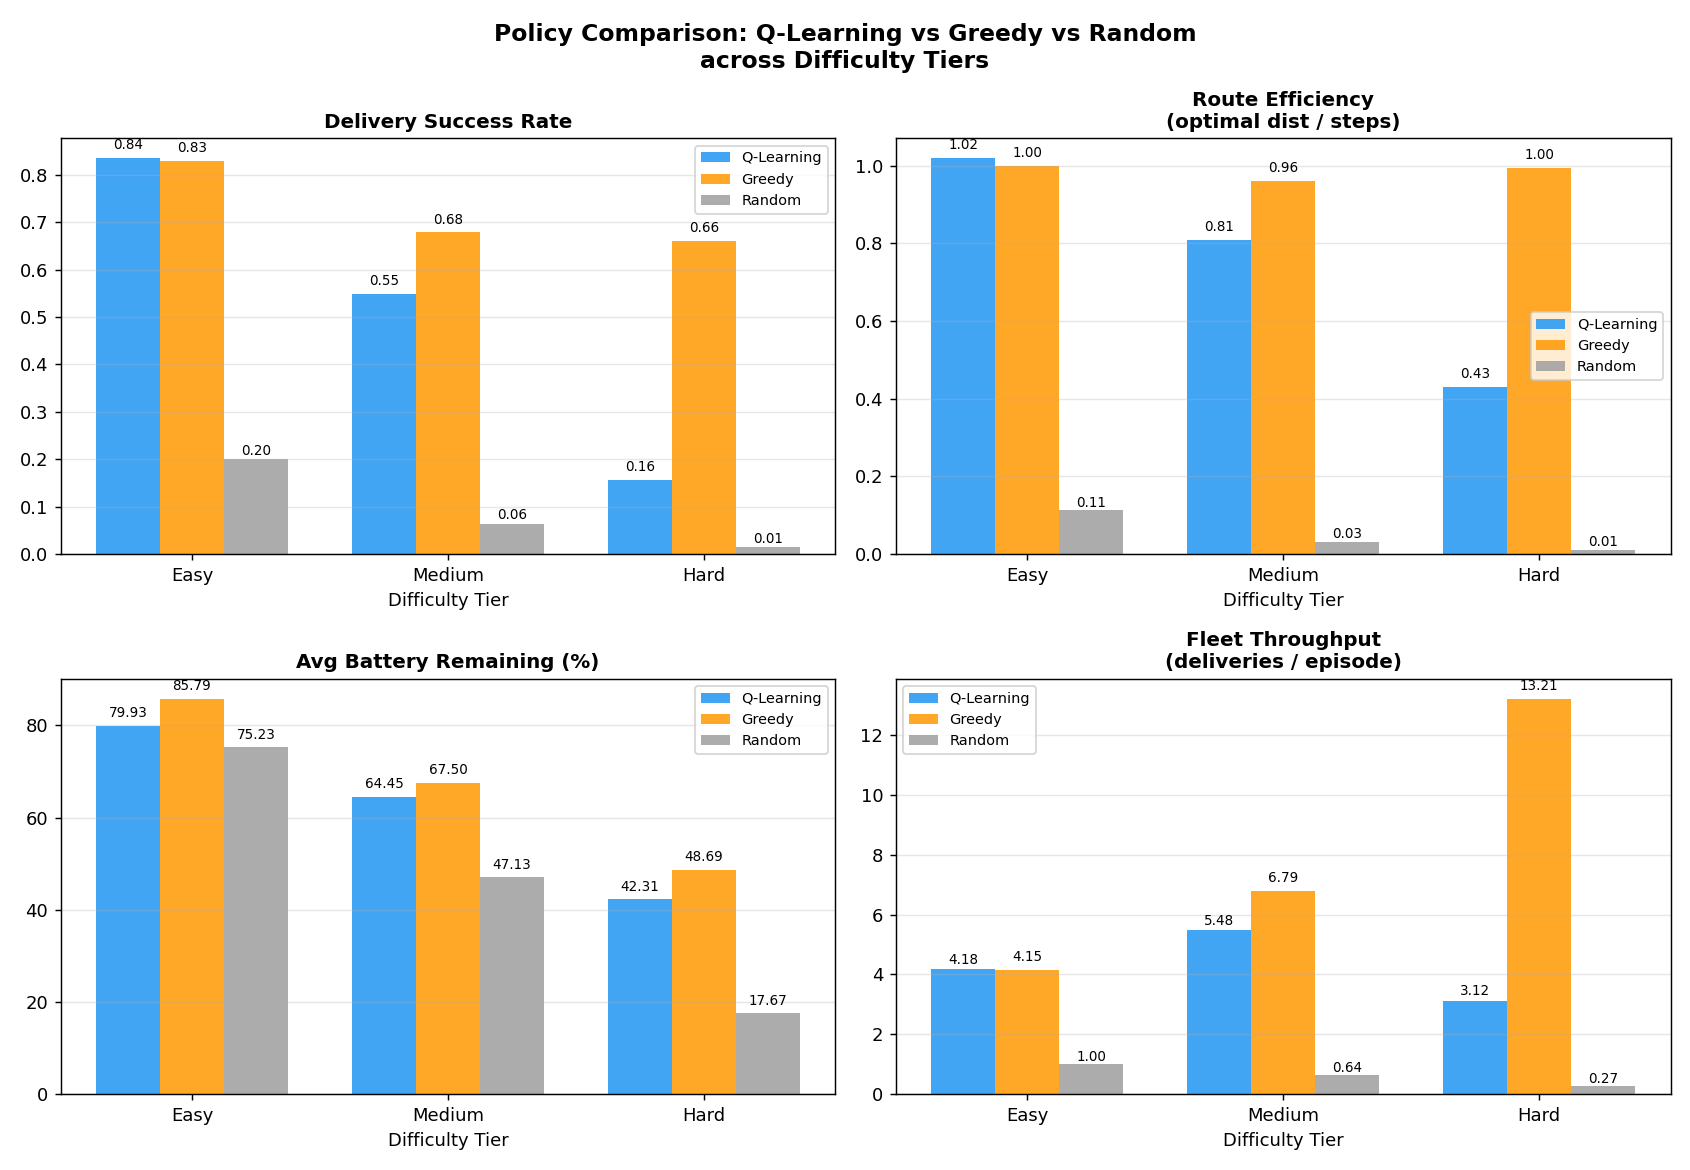
\includegraphics[width=\linewidth]{results.png}
    \caption{Bar chart of benchmark metrics. Q-Learning edges Greedy on
    easy but is surpassed on larger tiers.}
    \label{fig:barchart}
\end{figure}

\begin{figure}[H]
    \centering
    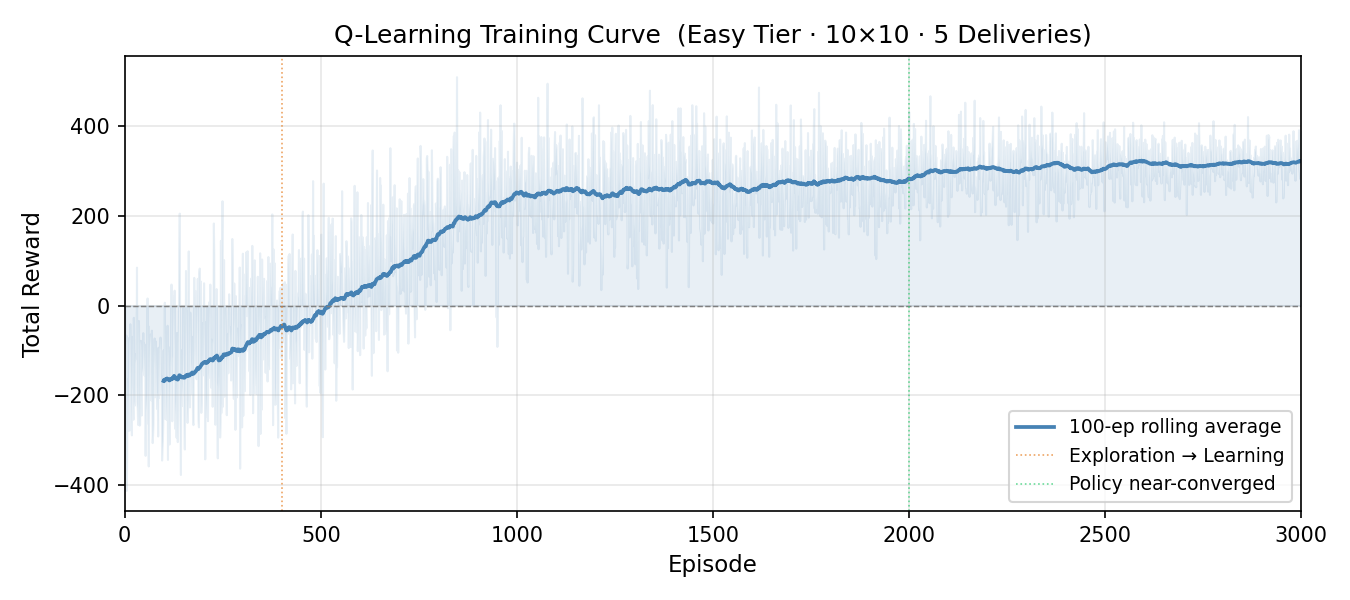
\includegraphics[width=\linewidth]{training_curve.png}
    \caption{100-episode rolling-average reward during Q-learning
    training (easy tier, 5\,000 episodes). The curve rises steeply
    during early exploration before plateauing as $\varepsilon$ decays.}
    \label{fig:training}
\end{figure}

% ─────────────────────────────────────────────────────────────────────────────
\section{Discussion}
\label{sec:discussion}
% ─────────────────────────────────────────────────────────────────────────────

\subsection{Q-Learning vs.\ Greedy on Easy Tier}

Q-learning achieves a delivery success rate of 83.5\% versus Greedy's
82.9\% on the easy tier, a difference of 0.6 percentage points.
While numerically small, this result is significant for two reasons.
First, the greedy policy embeds domain knowledge explicitly: it knows to
target the nearest delivery and to recharge below 20\%.
Q-learning acquires equivalent strategic intuition purely through
reward signals, without any hand-coded domain rules.
Second, Q-learning's route efficiency of 1.019 slightly exceeds Greedy's
1.000, suggesting the agent learns to sequence deliveries more cleverly
than a pure nearest-neighbour heuristic.

The marginal improvement also reflects a known weakness of tabular
Q-learning: with a sparse Q-table of approximately 663 visited states
after 5\,000 episodes, many unseen state--action pairs default to
$Q=0$, limiting the depth of learned strategy.
Additional training or a lower granularity state encoding could close
the gap further.

\subsection{Q-Learning Underperformance on Medium and Hard Tiers}

On medium (67.9\% vs.\ 54.8\%) and hard (66.1\% vs.\ 15.6\%) tiers,
Greedy substantially outperforms Q-learning.
This is a classic manifestation of the \emph{curse of dimensionality}
in tabular RL~\cite{bellman1957}.
As the grid grows from 10$\times$10 to 50$\times$50, the state space
expands dramatically: positions alone grow by a factor of 25, and the
\texttt{frozenset} of pending deliveries (20 items on hard) has
$2^{20} \approx 10^6$ possible values.
Our Q-table, trained only on easy scenarios, has never seen most of
these states and therefore falls back to $Q=0$, which is equivalent
to acting greedily with respect to the learned bias rather than the
true value.

Greedy, by contrast, is \emph{stateless}: its nearest-neighbour rule
transfers perfectly to larger grids because it depends only on
Euclidean distance, not on any learned representation.
This illustrates a fundamental trade-off in AI planning: learned
policies can surpass hand-coded heuristics when they have sufficient
training data, but they are vulnerable to distribution shift when
deployed in settings far outside their training distribution.

\subsection{The Role of A* in Both Layers}

A key insight from this project is that A* is not merely a helper
function---it is a first-class component of the agent's intelligence.
The greedy policy owes much of its strong performance to the fact that
it also uses A* implicitly: by always moving toward the nearest
delivery, it implicitly relies on A* reachability.
Q-learning's high-level decisions are only as good as the low-level
execution, and the quality of that execution depends entirely on A*'s
ability to find short, battery-efficient paths.

Dynamic replanning is particularly important on medium and hard tiers,
where 6--15 moving obstacles increase the probability that a planned
path becomes blocked mid-flight.
Without replanning, the drone would either stop (no action to take)
or proceed through an occupied cell (collision, $-50$ penalty).

\subsection{Battery Management}

An interesting secondary result is that Q-learning finishes episodes
with \emph{less} remaining battery than Greedy on every tier (e.g.,
79.9 vs.\ 85.8 on easy).
This suggests Q-learning makes more aggressive use of the battery
budget---it has learned that battery left over at the end of an episode
is wasted capacity that could have been spent on deliveries.
Greedy's 20\% recharge threshold is conservative; Q-learning has no
such hardcoded limit and will push the battery lower if its estimated
value of further deliveries justifies it.
On hard tier, Q-learning's more aggressive battery use contributes to
its lower success rate: more episodes end with a battery-out crash.

\subsection{The SKIP Action}

The inclusion of the \textsc{Skip} macro-action proved important for
learning a sensible policy.
Without it, the agent would have only two options---deliver or charge---
and would be forced to attempt every delivery regardless of feasibility.
In early training, the agent sometimes learns to skip deliveries that
are genuinely unreachable (insufficient battery, time window already
passed), which reduces crash penalties and increases the total reward
signal available for learning productive behaviour.

\subsection{Limitations and Future Work}

Several limitations are worth noting:

\begin{enumerate}[leftmargin=*, nosep]
    \item \textbf{State space coverage.}
          5\,000 training episodes on the easy tier leave the Q-table
          sparsely populated. Training on all three tiers simultaneously
          or using function approximation (e.g., a deep Q-network~\cite{mnih2015})
          would substantially improve medium/hard performance.
    \item \textbf{Partial observability.}
          The simulator is fully observable: the drone knows the
          positions of all obstacles and the wind map.
          In reality, these would be partially observable, requiring
          belief-state planning or recurrent policies.
    \item \textbf{Multi-drone coordination.}
          Our formulation uses a single drone. Extending to a fleet
          introduces cooperative planning challenges that would require
          multi-agent RL or centralised dispatch algorithms.
    \item \textbf{Continuous action space.}
          The 8-directional discrete action space is a significant
          simplification. Real drones navigate in continuous
          3-D space, suggesting a natural extension to continuous
          control methods.
\end{enumerate}

% ─────────────────────────────────────────────────────────────────────────────
\section{Baseline Comparison Summary}
\label{sec:baselines}
% ─────────────────────────────────────────────────────────────────────────────

Table~\ref{tab:baselines} provides a direct head-to-head comparison of
delivery success rate across all three policies and tiers.
Q-learning outperforms both baselines on the easy tier and all policies
outperform the random baseline by a wide margin on every tier,
validating that both the learned policy and the greedy heuristic
represent genuine planning intelligence over purely stochastic behaviour.

\begin{table}[H]
\centering
\small
\caption{Delivery success rate by policy and tier. $\Delta_{\text{QL}}$
is Q-Learning minus Greedy.}
\label{tab:baselines}
\begin{tabular}{lrrrc}
\toprule
\textbf{Tier} & \textbf{Q-Learn} & \textbf{Greedy} & \textbf{Random}
    & $\boldsymbol{\Delta_{\text{QL}}}$ \\
\midrule
Easy   & \textbf{83.5\%} & 82.9\% & 20.0\% & $+0.6\%$ \\
Medium & 54.8\%          & \textbf{67.9\%} & 6.4\%  & $-13.1\%$ \\
Hard   & 15.6\%          & \textbf{66.1\%} & 1.4\%  & $-50.5\%$ \\
\bottomrule
\end{tabular}
\end{table}

The degradation of Q-learning from easy ($+0.6\%$) to hard ($-50.5\%$)
relative to Greedy quantifies the distribution-shift problem discussed
in Section~\ref{sec:discussion}.
It also points directly toward the most impactful future improvement:
training the agent across all three tiers, or replacing the Q-table
with a neural network capable of generalising to unseen grid sizes.

% ─────────────────────────────────────────────────────────────────────────────
\section{Conclusion}
\label{sec:conclusion}
% ─────────────────────────────────────────────────────────────────────────────

We presented the Delivery Drone Route Planner, a two-layer autonomous
agent combining tabular Q-learning for high-level dispatch and A* search
for low-level path execution.
The system demonstrates that two classical AI paradigms---heuristic
search and reinforcement learning---can be composed into a coherent,
working agent that outperforms a hand-crafted baseline on the
distribution it was trained on (easy tier, 83.5\% success rate).

The project also surfaces fundamental lessons about the limits of
tabular RL: without sufficient state-space coverage, a learned policy
cannot generalise to harder settings, and a well-designed domain
heuristic can remain competitive.
This trade-off between learnability and generalisability is a central
theme in AI, and our results provide a concrete, reproducible
illustration of it.

All code, trained Q-tables, benchmark scenarios, and the interactive
Streamlit frontend are available in the project repository.

% ─────────────────────────────────────────────────────────────────────────────
\begin{thebibliography}{9}
% ─────────────────────────────────────────────────────────────────────────────

\bibitem{hart1968}
P.~E. Hart, N.~J. Nilsson, and B.~Raphael,
``A formal basis for the heuristic determination of minimum cost paths,''
\textit{IEEE Trans.\ Syst.\ Sci.\ Cybern.}, vol.~4, no.~2,
pp.~100--107, 1968.

\bibitem{watkins1992}
C.~J. C.~H. Watkins and P.~Dayan,
``Q-learning,''
\textit{Machine Learning}, vol.~8, no.~3--4,
pp.~279--292, 1992.

\bibitem{bellman1957}
R.~Bellman,
\textit{Dynamic Programming}.
Princeton University Press, 1957.

\bibitem{mnih2015}
V.~Mnih \textit{et al.},
``Human-level control through deep reinforcement learning,''
\textit{Nature}, vol.~518, pp.~529--533, 2015.

\bibitem{likhachev2005}
M.~Likhachev, D.~Ferguson, G.~Gordon, A.~Stentz, and S.~Thrun,
``Anytime dynamic A*: An anytime, replanning algorithm,''
\textit{Proc.\ ICAPS}, pp.~262--271, 2005.

\bibitem{sutton2018}
R.~S. Sutton and A.~G. Barto,
\textit{Reinforcement Learning: An Introduction}, 2nd ed.
MIT Press, 2018.

\end{thebibliography}

\end{document}
